f\chapter{Introduction}

\setlength{\parindent}{4em}
\setlength{\parskip}{1em}
\renewcommand{\baselinestretch}{1.5}
\section{Motivation}

\hspace{1.5cm}Nowadays, The technology is used for the advantages in many fields, for example, an ultrasound machine in the medical field, a soil and crop sensor in the agriculture field, a robotic arm for move the product in industry field and also the several technologies for a facility in daily life. At present, one of the technologies which are interesting and important is technology to improve a quality of life of the disabilities. The invention of equipment which can be interacted by using non-muscular communication channel can help these kinds of people in daily life or in the emergency.\par
For those people with physical or mobile impairment, one of the common problems in daily life is that they cannot completely control equipment that is designed for ordinary people. Making the equipment for the disabled people to help them can be interacted or communicated by using brain signal instead of muscle that is one of the choices to solve their problem. The technology that obtains the brain signal and translates the brain signal to communicate or interact with the external device is called Brain-Computer Interface (BCI). At present, there are three types of BCI, divided by the stimulation : Auditory BCI Imaginary BCI and Visual BCI. Each type has the different advantages and disadvantages. First is the auditory BCI that is easy to analyze the brain signal but it has slow interpretation and the sound from this BCI can annoy other people. Next, imaginary BCI is the fastest way to stimulate the brain but the subject should be trained before using this BCI and it has a low rate of success. The last one is visual BCI that is the easiest way to obtain the brain signal However, it cannot use in case of the epilepsy person.\par
Our project will use the visual type of Brain-Computer Interface to control the application for the disabled people. We use brain signal from the subject to control programs or devices. When the user was stimulated by the flicker, the brain will generate waveform and be the different pattern from others.  

\section{Objective}
\hspace{1.5cm} The objective of this project is to make the user able to communicate or interact with our equipment by using brainwave. This can help the disabled people when they need some emergency or facilities. \par
Furthermore, our purpose is to study various techniques to record and translate the brainwave to interact with the external devices. 

\section{Scope of work}

The scope of this project can be summarized as follows:
%write more scope of work
\begin{itemize}
\vspace{-1cm}
	\item Study the theories and techniques of recording EEG waveform.
\vspace{-1cm}
    \item Make an equipment which a user can cognitively interact or use the system by brain-wave without using muscle function.
\end{itemize}  

\section{Contributions}
\hspace{1.5cm} In this project, we have developed a control module for users to interact with software by using EEG signal. Our work demonstrates a brand new alternative way to help users in a more convenient way or help immobilize-able users with limited control on their parts of the body. We hope that a control module and software that we have developed will provide great advantages and only minor disadvantages to the project.

\section{Procedure}
We separate that work into 6 phases. 
\begin{enumerate}
\vspace{-0.5cm}
\item Plan the project 
\vspace{-0.25cm}
\item Research and study on EEG cognitive 
\vspace{-0.25cm}
\item Design the equipment 
\vspace{-0.25cm}
\item Implement the system 
\vspace{-0.25cm}
\item Doing an experiment 
\vspace{-0.25cm}
\item Testing program
\end{enumerate}

\newpage

\begin{figure}[ht]
	\centering
	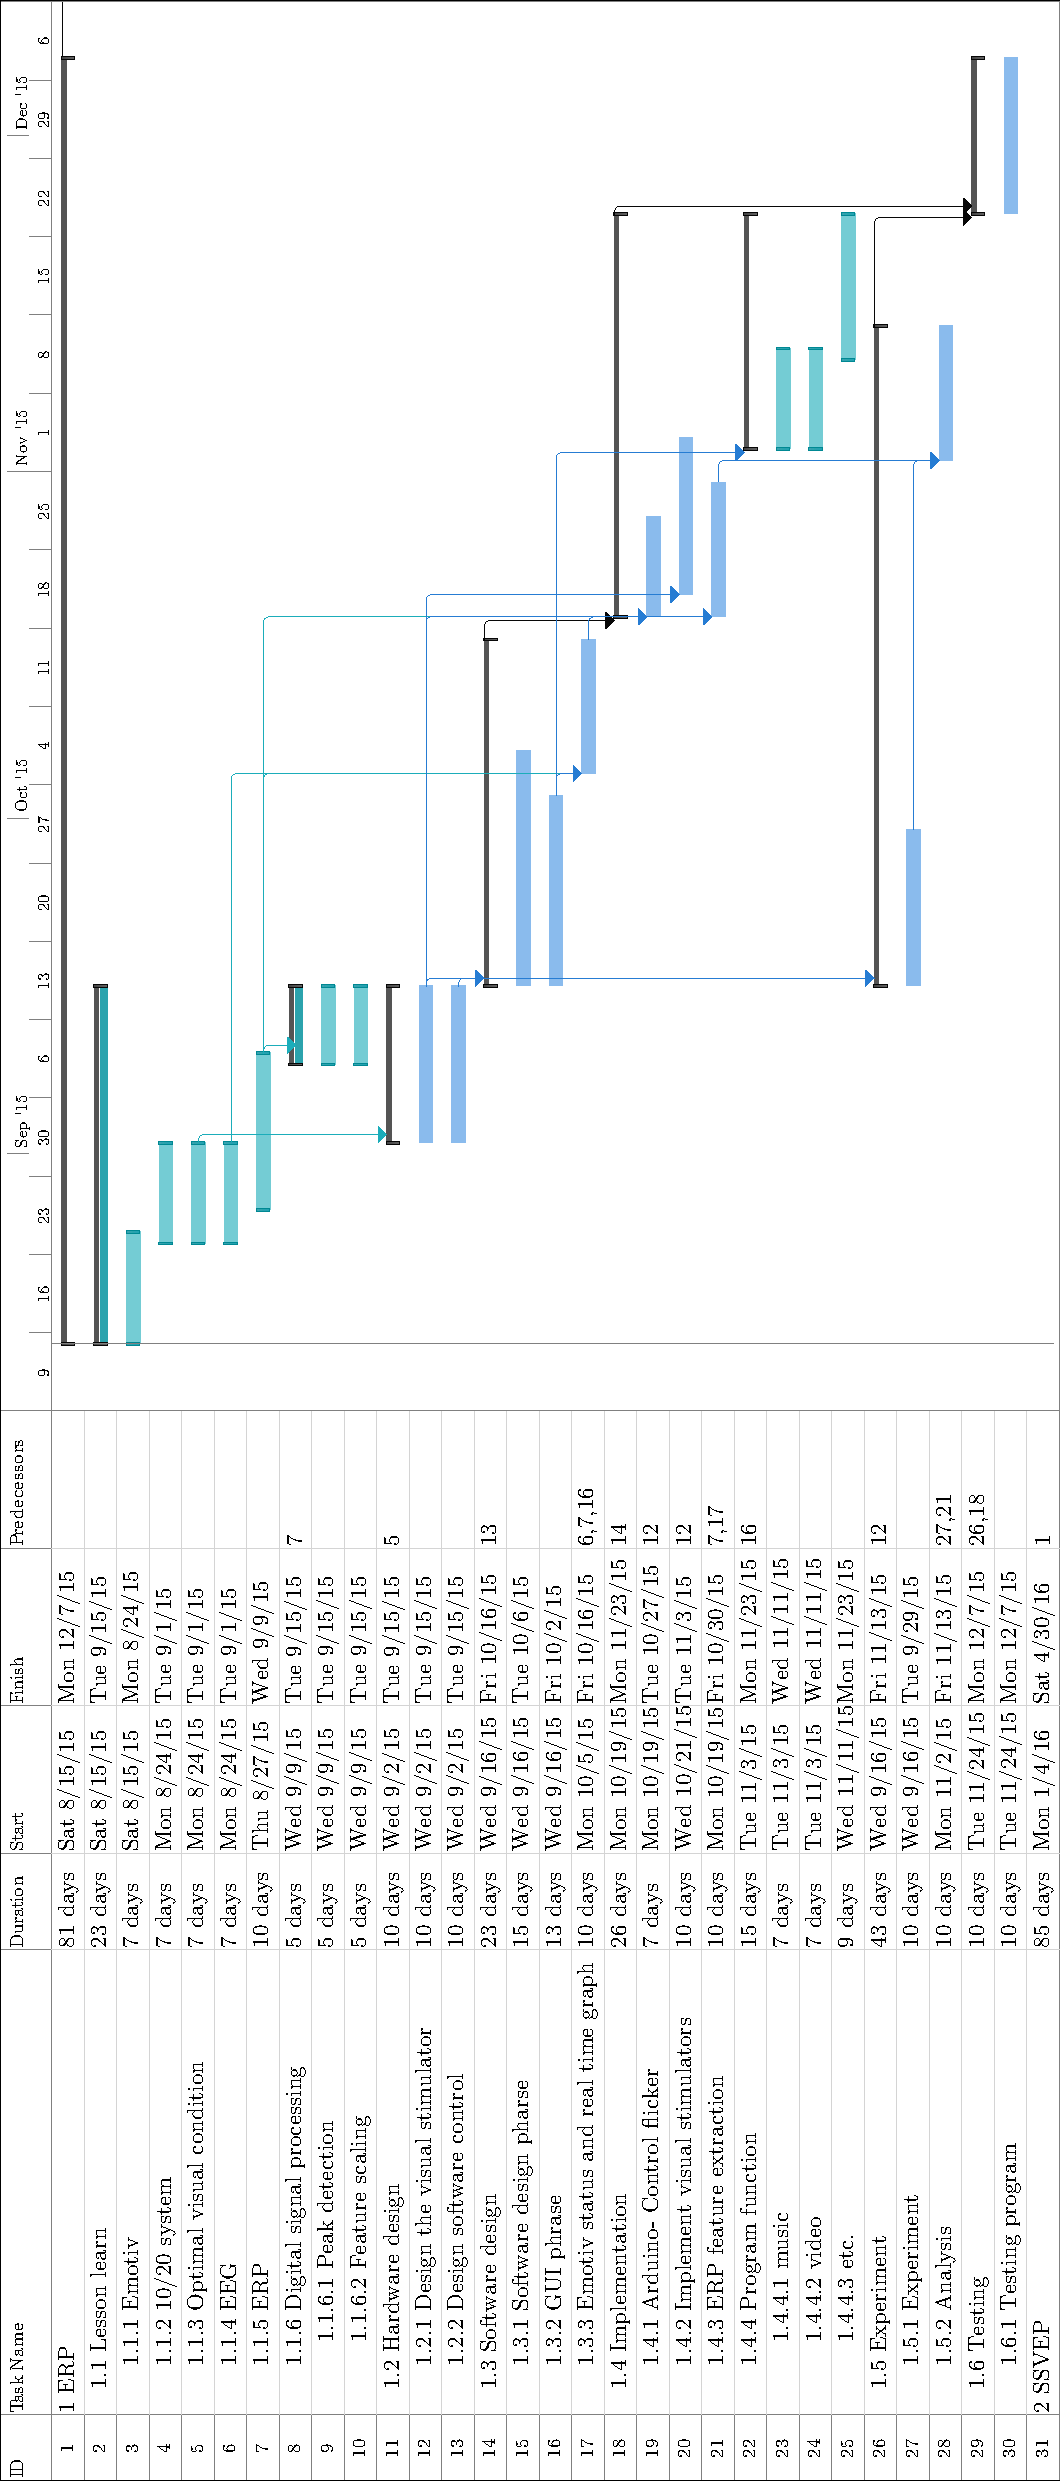
\includegraphics[\textwidth]{chapter1/gan1.pdf}
	\caption{The subject control robot use brain wave and communicate via camera at same time}
\end{figure}

\begin{figure}[ht]
	\centering
	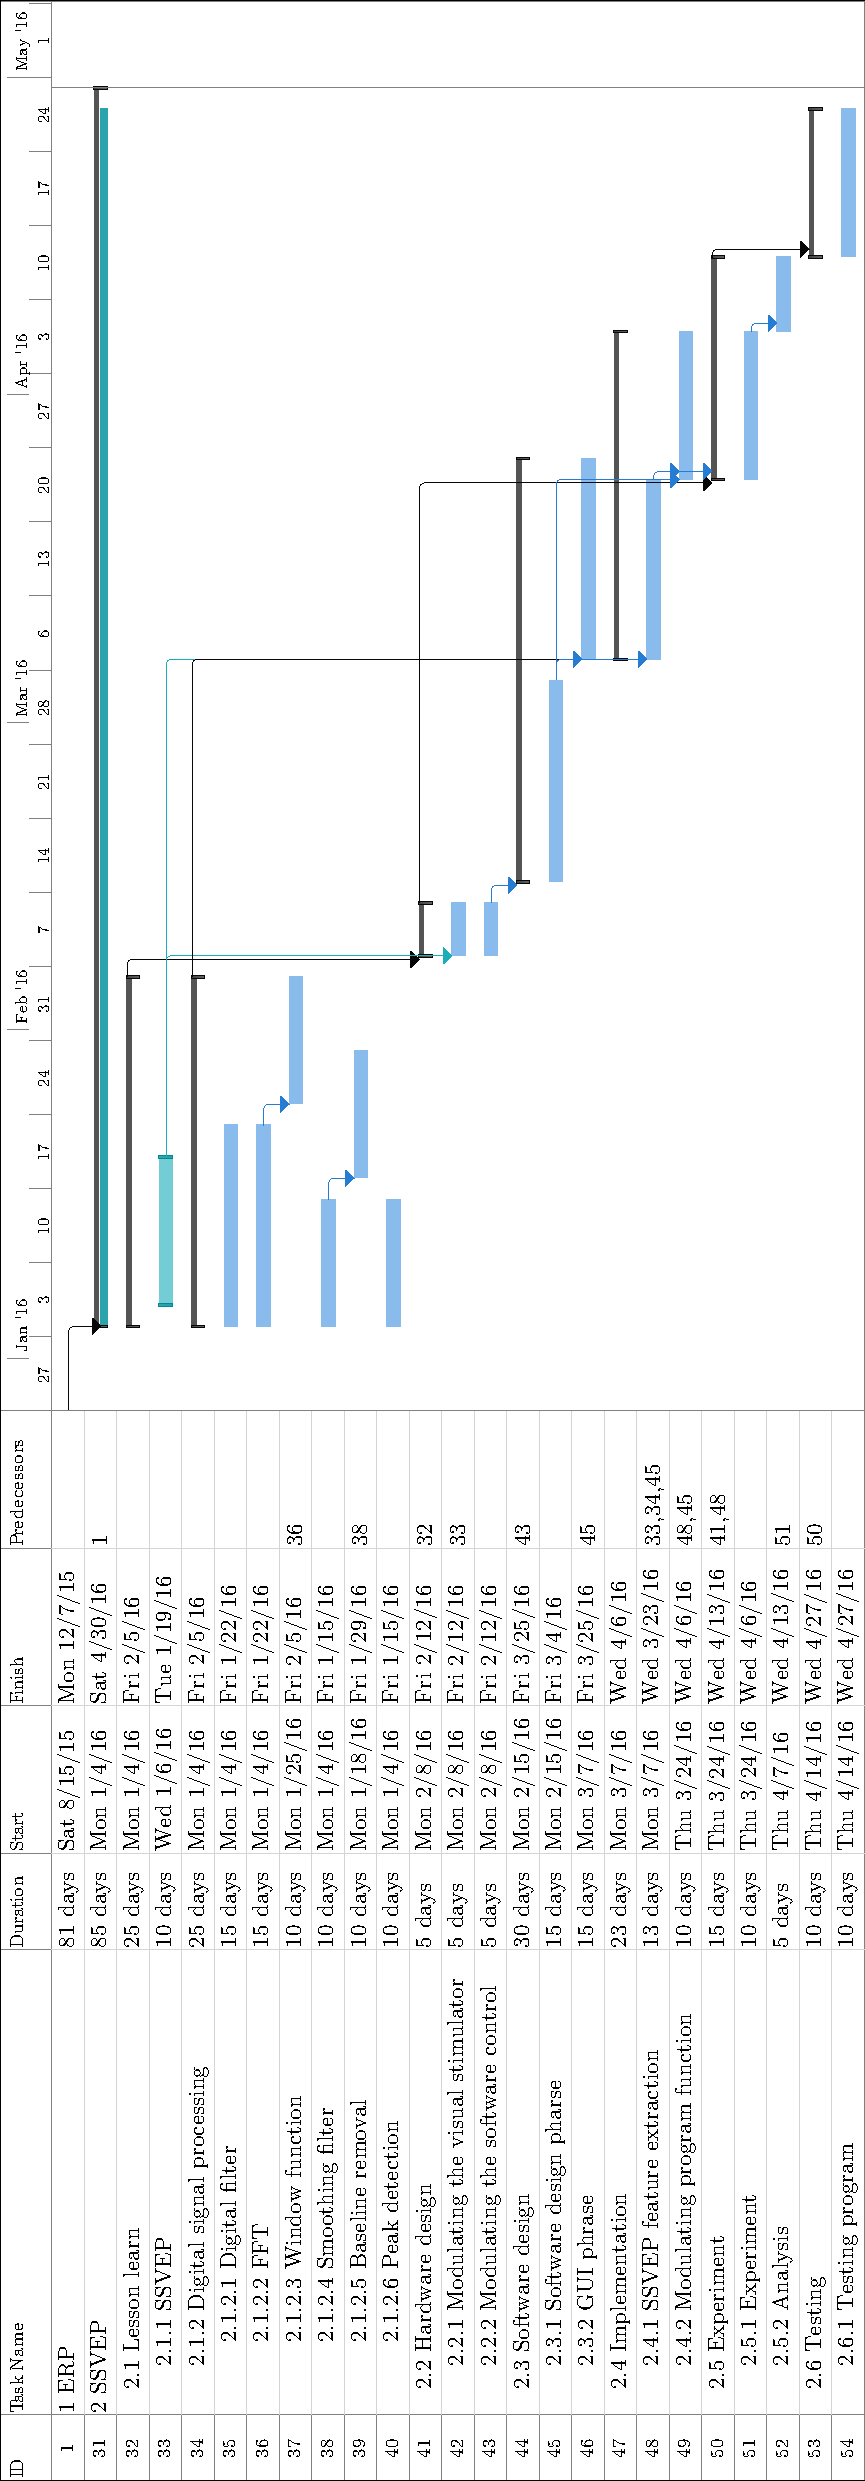
\includegraphics[scale = 0.4]{chapter1/gan2.pdf}
	\caption{The subject control robot use brain wave and communicate via camera at same time}
\end{figure}

